\documentclass[output=paper]{langsci/langscibook} 
\author{Christopher Lucas\affiliation{SOAS University of London}\lastand 
 Stefano Manfredi\affiliation{CNRS, SeDyL}
}
\title{Introduction}
% \keywords{} 
\abstract{Abstract}
\maketitle

\begin{document}\label{introintro}

\section{Purpose of the volume}
With its lengthy written history, wide and well-studied dialectal variation, and involvement in numerous heterogeneous contact situations, the Arabic language has an enormous contribution to make to our understanding of how language contact can lead to change. Until now, however, most of what is known about the diverse outcomes of contacts between Arabic and other languages has remained inaccessible to non-specialists. There are brief summary sketches \citep{Thomason2011,Versteegh2001article,Versteegh2010,Manfredi2018}, as well as a recent collection of articles on a range of issues connected with Arabic and language contact in general \citep{ManfrediTosco2018}, but no larger synthesis of the kind that is available, for example, for Amazonian languages \citep{Aikhenvald2002}.

Arabic has thus played little part in work to date on contact-induced change that is crosslinguistic in
scope (though see \citealt{Matras2009,Trudgill2011} for partial exceptions). By providing the community of general and historical linguists with the present collaborative synthesis of expertise on Arabic and contact-induced change, we hope to help rectify this situation. The work consists of twenty-nine chapters by leading authorities in their fields, and is divided into three Parts: overviews of contact-induced change in individual Arabic varieties (Part I); overviews of the outcomes of contact with Arabic in other languages (Part II); and overviews of various types of changes across Arabic varieties, in which contact has played a significant role (Part III). Chapters in each of the three Parts follow the fixed broad outlines detailed below in §\ref{introstructure}, in order to maximize coherence and ease of reference. All authors have also been encouraged a) to ensure their chapters contain a rich set of (uniformly glossed and transcribed) linguistic data, including original data where appropriate, and b) to provide as much sociohistorical data as possible on the speech communities involved, framed where possible with reference to Van Coetsem’s (\citeyear{VanCoetsem1988,VanCoetsem2000}) distinction between changes due to borrowing (by agents dominant in the recipient language) and imposition (by agents dominant in the source language; see §\ref{introvc} for further details). These features are aimed at ensuring that the data presented in the volume can be productively drawn upon by scholars and students of linguistics who are not specialists in
Arabic linguists, and especially those working on the mechanisms, typology, outcomes, and theory of contact-induced change cross-linguistically. 

Inevitably with a project of this scale, it has not been possible to cover every  aspect of the topic that we would have liked to, and the chapters included necessarily represent a compromise between several different academic and practical considerations. For instance, we have aimed for blanket coverage of languages and varieties of Arabic that have been significantly affected by contact, but for some varieties (e.g. Yemeni Arabic dialects) it was not possible to recruit a scholar with sufficient expertise to contribute a chapter. Where blanket coverage has not been possible, we have generally sought to focus on those individual varieties and dialect areas that have been most intensively affected by contact (e.g. Maltese, Maghrebi Arabic in general, Domari), while not also excluding languages and varieties where contact influence has been milder (e.g. Beja, Iranian languages, Classical and Modern Standard Arabic), but for which we could source experts ready to contribute chapters.

The rest of this introduction is structured as follows. 




\section{Existing work on Arabic and contact-induced change}\label{introexistingwork}

\begin{itemize}[noitemsep]

\item[] Brief overview works already mentioned in §\ref{introintro}: \citet{Thomason2011}, \citet{Versteegh2001article,Versteegh2010}, \citet{Manfredi2018}

\item[]Comparative works on several Arabic varieties: \citet{Owens2018}

\item[]Yemen/MSAL/South Arabian: \citet{Diem1979}, \citet{Watson2018}

\item[]Works on contact influences on Classical and Modern Standard Arabic: \citet{Jeffrey2007} [1938], \citet{Blau1969}, \citet{Hebbo1984}

\item[]Nabataea: \citet{Macdonald2003}

\item[]Arabic and Aramaic: \citet{Fraenkel1886}, \citet{Stein2018}, \citet{Retsö2011}, \citet{Weninger2011Aramaic}

\item[]Arabic and Neo-Aramaic:
\citet{ArnoldBehnstedt1993} \citet{Borg2008}, \citet{Coghill2012,Coghill2015}, \citet{Jastrow2015}, \citet{Owens2016Aramaic}

\item[]Arabic and Hebrew:
\citet{Blau1981}, \citet{Nevo1999}, \citet{Yoda2013}

\item[]Arabic and Ethio-Semitic: \citet{Nöldeke1910}

\item[]Arabic and Greek: \citet{Gutas2011},

\item[]Arabic and Persian: \citet{Asbaghi2011}, \citet{Gazsi2011}

\item[]Arabic and Turkish: \citet{BenCheneb1922}, \citet{Reinkowski1995}, \citet{Procházka2002Adana,Procházka2011Turkish}, \citet{Isaksson2005}, \citet{SánchezVicente2012}, \citet{Haig2014}, \citet{Taylan2017}, \citet{AkkusBenmamoun2018}, \citet{Procházka-Eisl2018}

\item[]Arabic and Berber: \citet{Corriente1981, Corriente1998Berber,Corriente2002}, \citet{Taine-Cheikh1997Zenaga,Taine-Cheikh2008chapter,Taine-Cheikh2018quadri}, \citet{Brahimi2000}, \citet{Ameur2008},
\citet{Kossmann2009,Kossmann2010,Kossmann2013book,Kossmann2013chapter,Kossmann2014}, \citet{Souag2007,Souag2009,Souag2013book,Souag2018berber,Souag2018thing}, \citet{Lafkioui2013reinventing,Lafkioui2013bu}, \citet{Tigziri2008}, \citet{vanPuttenBenkato2017}

\item[]Arabic and (sub-)Saharan languages: \citet{Owens2000article,Owens2015,Owens2016idioms}, \citet{OwensHassan2004} \citet{Souag2013lexical,Souag2016sahara}

\item[]Arabic and Latin/Romance languages: \citet{Brunot1949}, \citet{Benoliel1977}, \citet{Corriente1978,Corriente1992chapter,Corriente1992book,Corriente1995,Corriente2000,Corriente2005,Corriente2008}, \citet{Talmoudi1986}, \citet{Abdu1988}, \citet{Heath1989,Heath1999,Heath2015}, \citet{Cifoletti1994}, \citet{Ferrando1995,Ferrando1997}, \citet{OuldMohamedBaba2003}, \citet{Vicente2006},
\citet{Sayahi2011,Sayahi2014,Sayahi2015}, \citet{Danna2018phonetic}

\item[]Contact influence in Maltese: \citet{colin1957}, \citet{Aquilina1958}, \citet{krier1976}, \citet{Drewes1994}, \citet{mifsudloanverbs}, \citet{stolz2003}, \citet{vella2003}, \citet{bovingdondalli2006}, \citet{brincat1996,brincat2011}, \citet{comriespagnol2016}, \citet{dohla2016}, \citet{Souag2018berber}

\item[]Contact influence in eastern Arabia/Arabian Gulf: \citet{Holes2002}

\item[]Contact influence in Mesopotamian Arabic: \citet{Masliyah1996,Masliyah1997}, \citet{Ingham2005}, \citet{Shabibi2006}, \citet{MatrasShabibi2007}, \citet{ElZarkaZiagos2019}

\item[]Contact influence in Levantine Arabic: \citet{Barbot1961}, \citet{Halasi-Kun1969,Halasi-Kun1973,Halasi-Kun1982}, \citet{Hopkins1995}, \citet{Contini1999}, \citet{Horesh2015}, \citet{Neishtadt2015}, 

\item[]Contact influence in Cypriot Arabic: \citet{Newton1964}, \citet{Tsiapera1964}, \citet{Borg1985,Borg1997CMA,Borg2004}, \citet{Roth2004}, \citet{Gulle2016} 

\item[]Contact influence in Central Asian Arabic: \citet{Ratcliffe2005}, \citet{Ingham2011afg}, \citet{Jastrow2005}

\item[]Arabic pidgins and creoles: \citet{Owens1985}, \citet{BurengVincent1986}, \citet{Miller1989,Miller1993}, \citet{Nakao2012}, \citet{Luffin2014}, \citet{Manfredi2014relex}, \citet{Avram2017article,Avram2019} \citet{Bizri2018}

\item[]Contact between Arabic dialects: \citet{Behnstedt1994Dialektkontakt}, \citet{Gibson2002}, the contributions to \citet{Miller2007}, \citet{Palva2009}, \citet{Vicente2010}

\item[]Differential object marking: \citet{Coghill2014}, \citet{Souag2017clitic}

\item[]Negation: \citet{Lucas2007,Lucas2012,Lucas2013}, \citet{LucasLash2010}, \citet{BreitbarthWillisLucasinpress}


\end{itemize}

\section{A dominance-based approach to contact-induced change}\label{introvc}
Introduce Van Coetsem's model.

\subsection{Imposition}
Example changes in the volume that are SL-agentivity based

\subsection{Borrowing}
Example changes in the volume that are RL-agentivity based

\subsection{Problematic cases}
...

\section{Alternative approaches to contact-induced change}\label{introotherapproaches} 
...

\section{What and where is Arabic?}

\begin{figure}
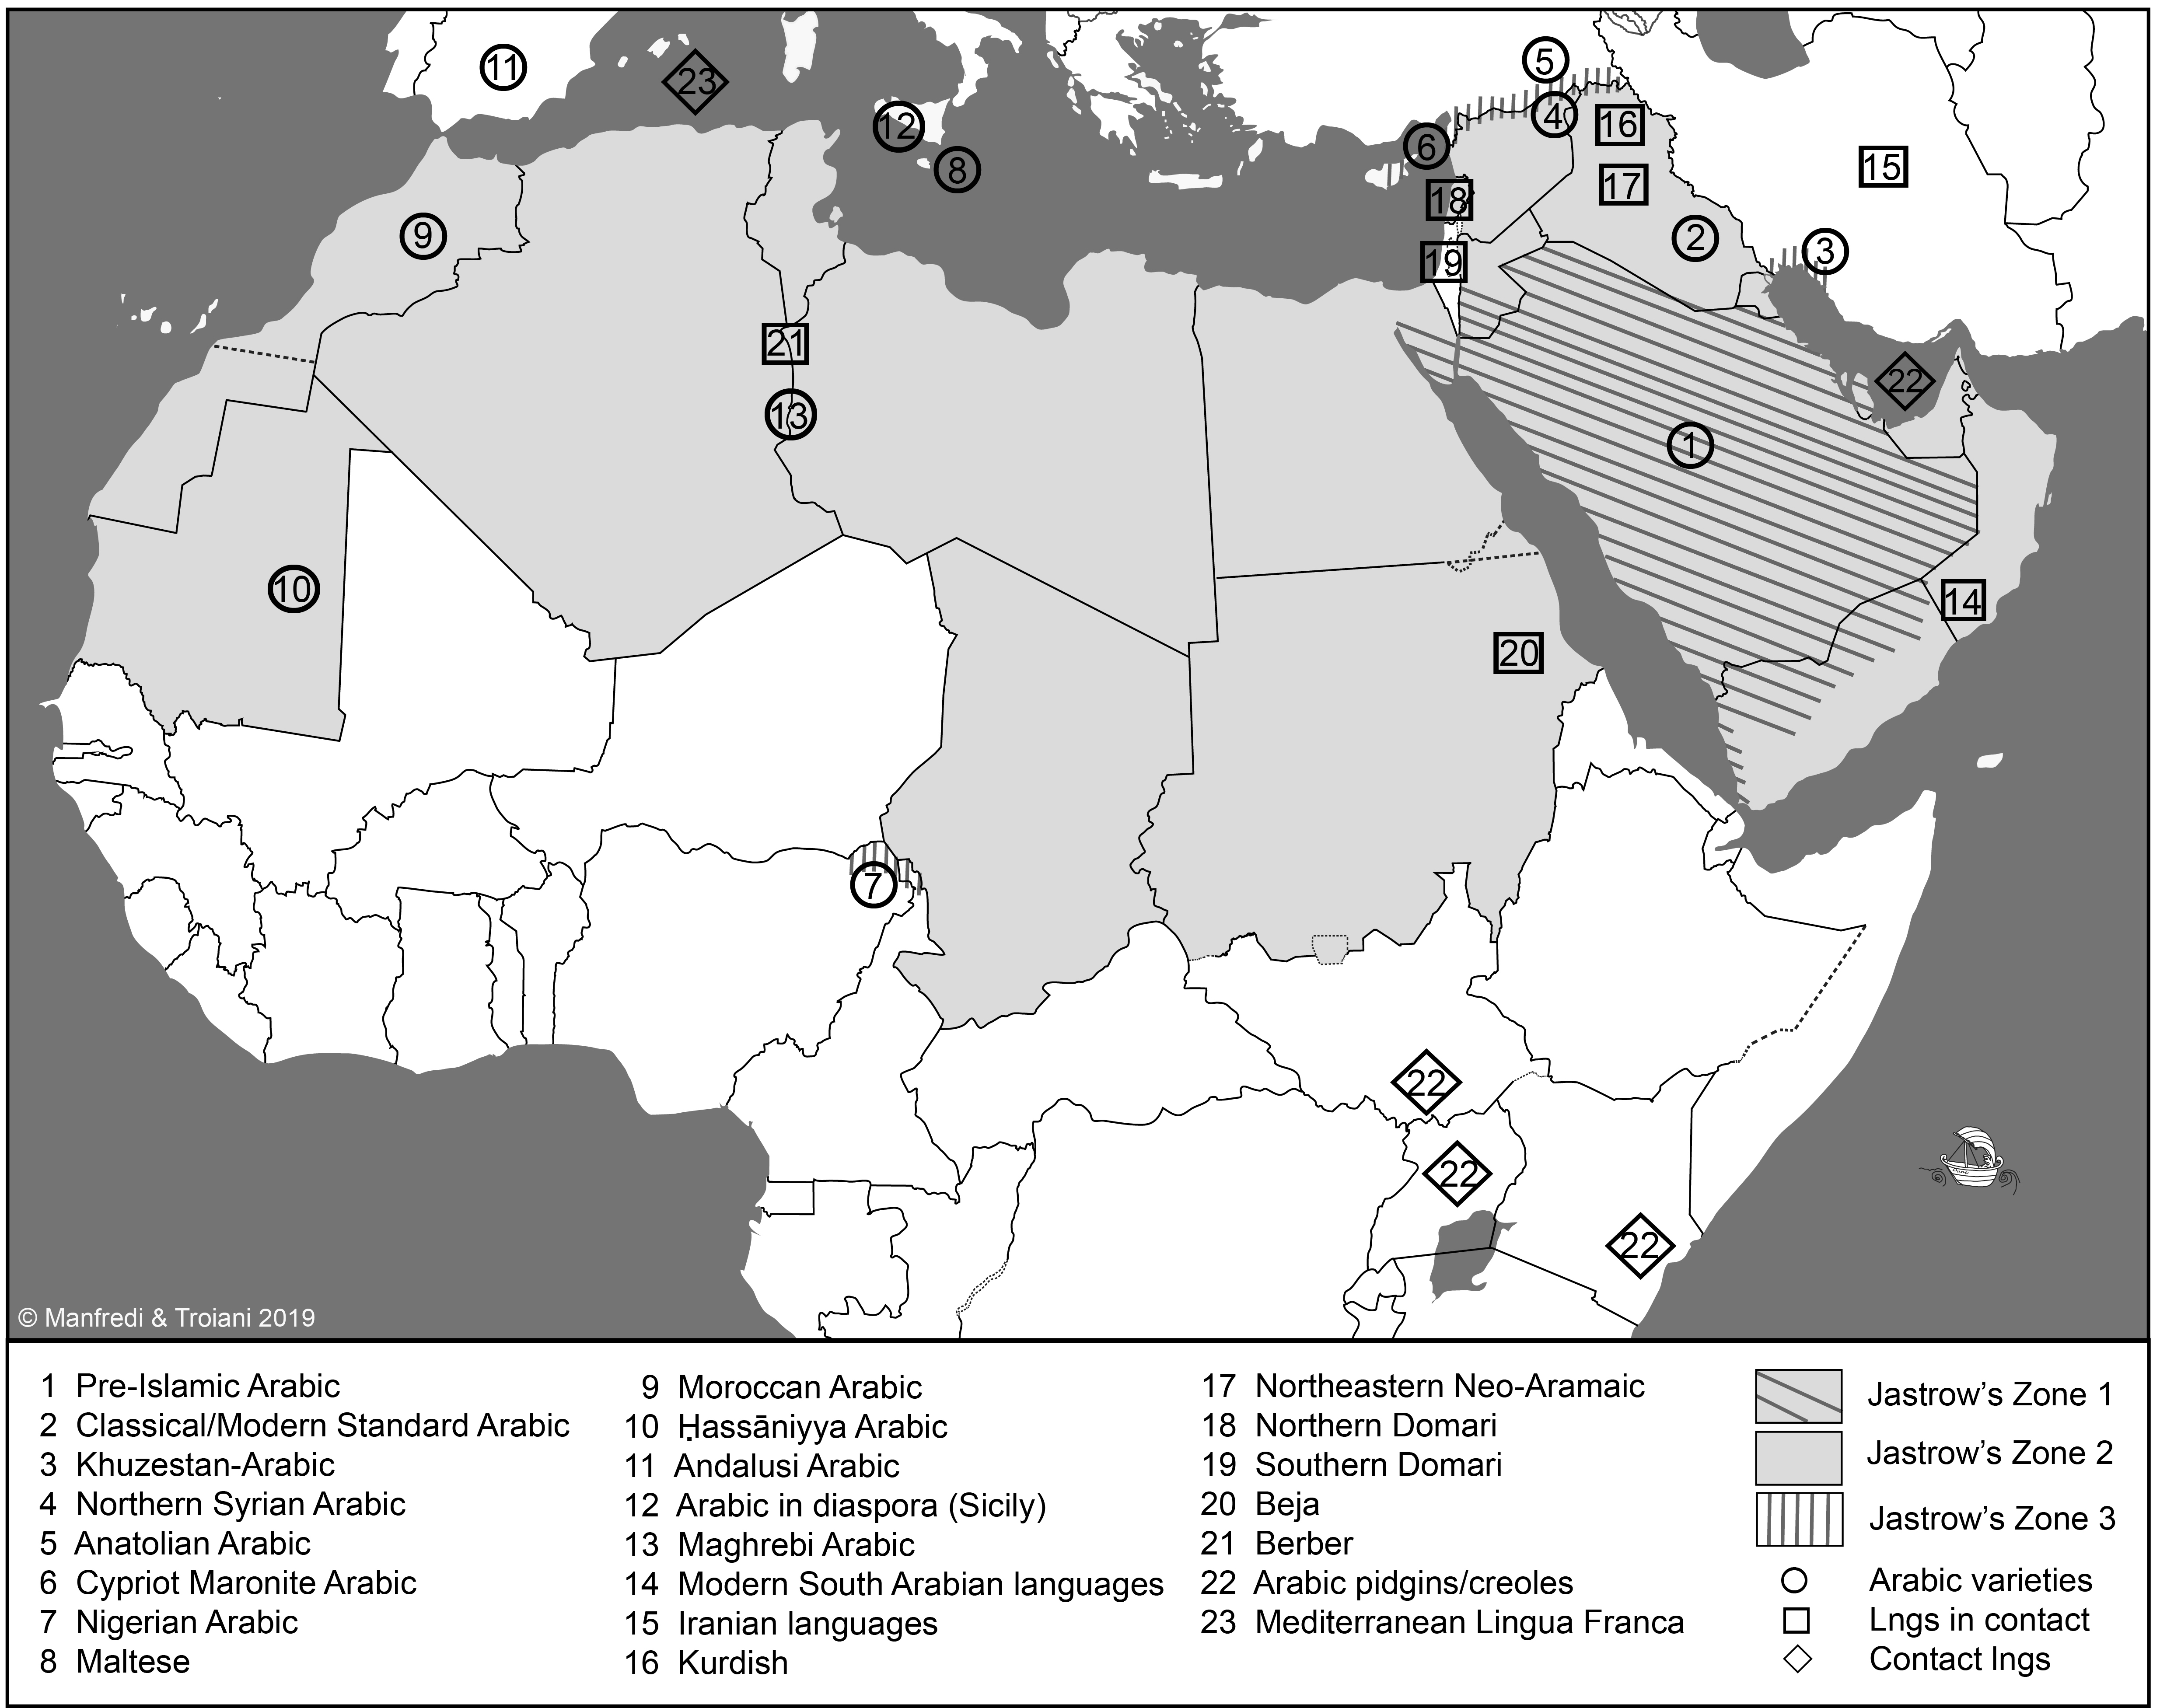
\includegraphics[width=\textwidth]{figures/Monde_arabe.jpg}
\caption{Map small and standard orientation}
\label{intromap}
\end{figure}

...
  
\begin{figure}
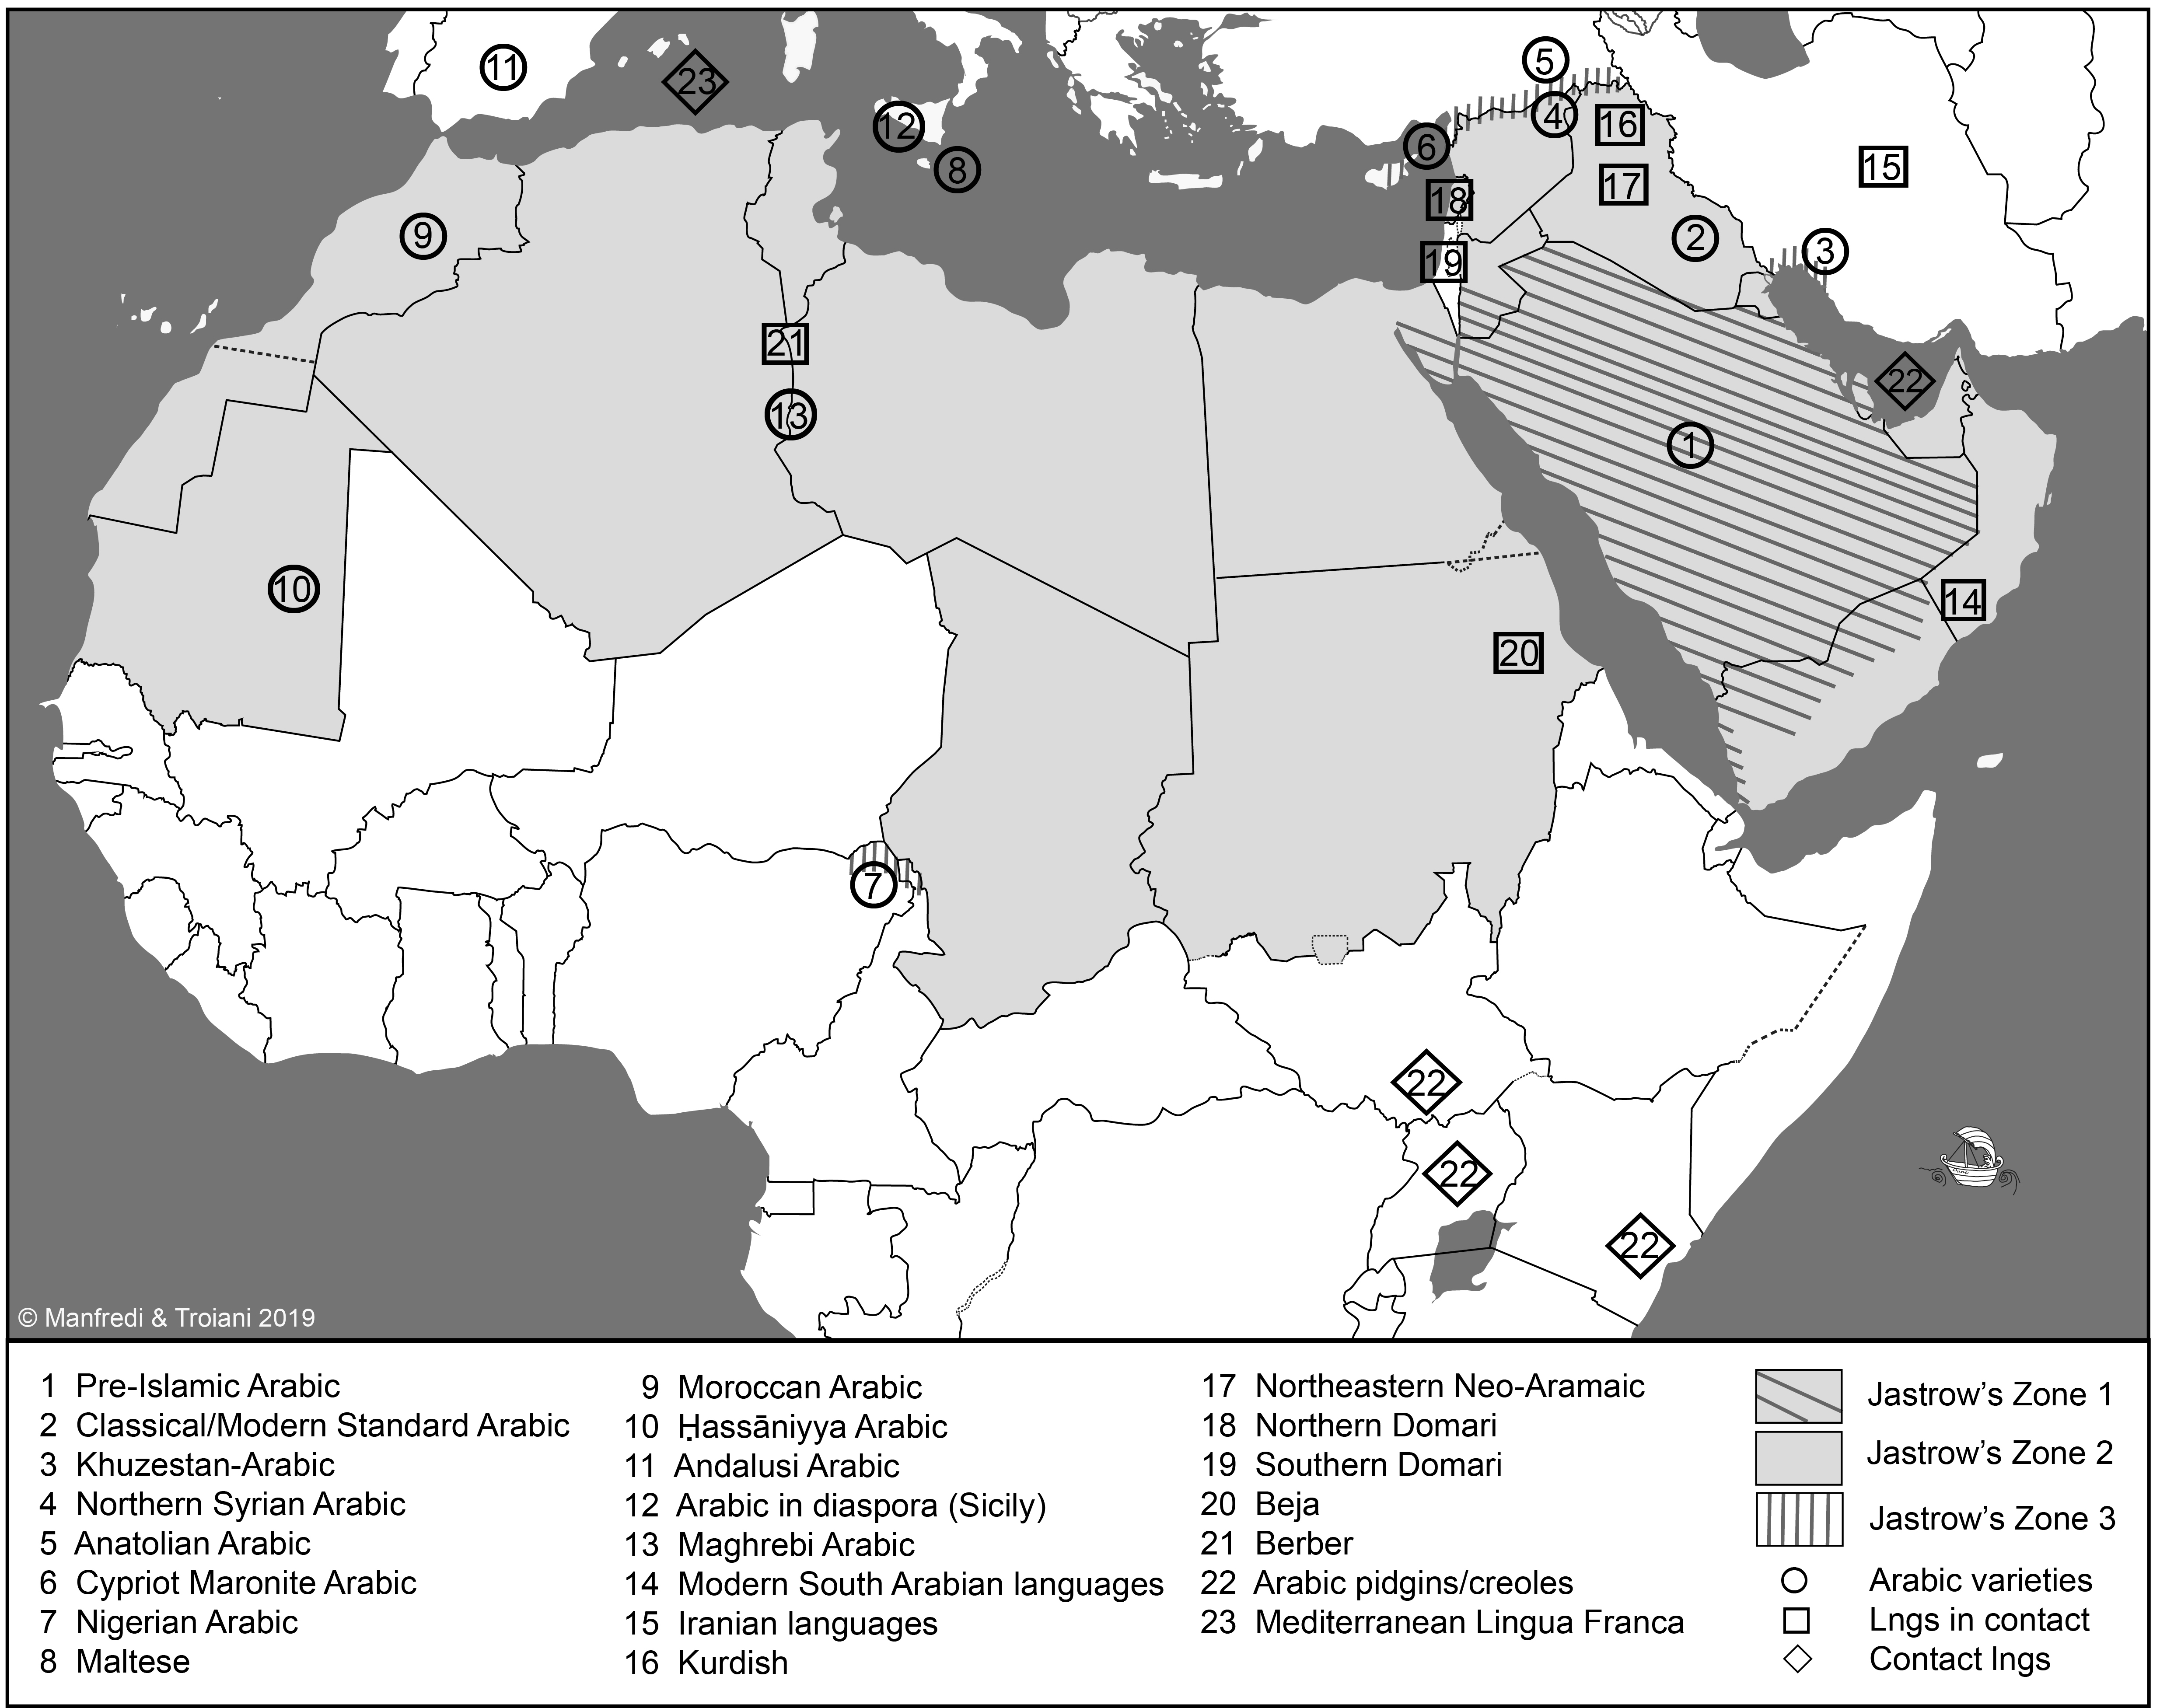
\includegraphics[height=.66\textheight, angle=90]{figures/Monde_arabe.jpg}
\caption{Map large and rotated orientation.}
\label{intromaplarge}
\end{figure}


\section{Languages in contact with Arabic}\label{introcontactlans}
...

\section{The structure of the present work}\label{introstructure}
...

\section{Major themes of the present work}\label{introthemes}
...

\section{Future directions}\label{introfuture}
...

\section*{Abbreviations}

Some references:\\
\\
\citet{Jastrow2002}\\
\citet{Owens2000editor}\\
\citet{Watson2011dialectsoverview}



\sloppy
\printbibliography[heading=subbibliography,notkeyword=this] 
\end{document}